% Kapitel 4 mit den entsprechenden Unterkapiteln
% Die Unterkapitel können auch in separaten Dateien stehen,
% die dann mit dem \include-Befehl eingebunden werden.
%-------------------------------------------------------------------------------
\chapter{Datenmodell}
Der Achterbahn-Simulator liest die Daten für die Achterbahn aus einer XML-Datei
mit vorgegeben XSD-Schema. Zum Auslesen der Angaben wird die XML-Datei deserialisiert.
Dafür kommt die Bibliothek JAX-B zum Einsatz, welche eine Anbildung der XML-Struktur
auf eine Klassenhierachie bereitstellt und zur Laufzeit entsprechend befüllt.

\section{Diagramm}

\begin{figure}
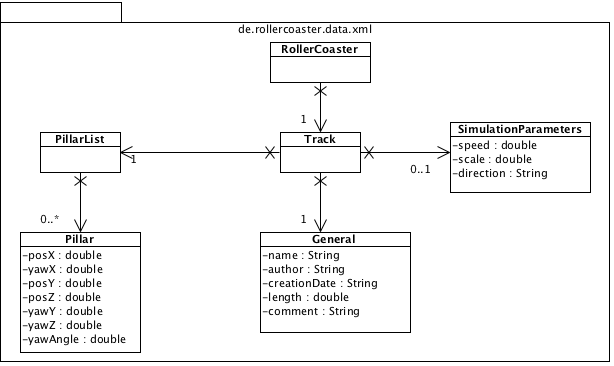
\includegraphics[width=\linewidth]{bilder/XML.png}
\caption{Deserialisiertes Schema für den Achterbahnsimulator}
\label{fig:xml}
\end{figure}

\section{Erläuterung}
Die Tabelle ist um so viele Einträge zu erweitern, wie es Entities im obigen
ER-Modell gibt. Für jedes Entity sind so viele Einträge in der
Beziehungs-Subtabelle einzufügen, wie es Beziehungen zu diesem Entity gibt.


\begin{tabular}[ht]{|l|c|}
  \hline
  Entität & Beziehungen\\
  \hline\hline
  <Entity … ID>:  & Name der Beziehung |  Kardinalität\\
  \hline\hline\hline
  <Bezeichnung> & <Name der Beziehung> | <Kardinalität>\\
  \hline
\end{tabular}
